\documentclass[12pt]{article}
\usepackage{graphics}
\usepackage{graphicx}
\usepackage{listings}
\usepackage{float}

\title{Datascience Homework 5}
\author{Ali Asghar Yousuf - ay06993}
\date{\today}

\begin{document}
\maketitle
\section{Table Creation}
\subsection{EmployeeAttrition1}
\begin{lstlisting}
CREATE TABLE EmployeeAttrition1(
	EmployeeNumber INT,
	Age INT,
	BusinessTravel VARCHAR(255),
	DailyRate INT,
	Department VARCHAR(255),
	DistanceFromHome INT,
	Education INT,
	EducationField VARCHAR(255),
	EnvironmentSatisfaction INT,
	Gender VARCHAR(255),
	HourlyRate INT,
	JobInvolvement INT,
	JobLevel INT,
	JobRole VARCHAR(255),
	JobSatisfaction INT,
	MaritalStatus VARCHAR(255),
	MonthlyIncome INT,
	MonthlyRate INT,
	NumCompaniesWorked INT,
	PercentSalaryHike INT,
	PerformanceRating INT,
	RelationshipSatisfaction INT,
	StandardHours INT,
	StockOptionLevel INT,
	TotalWorkingYears INT,
	TrainingTimesLastYear INT,
	WorkLifeBalance INT,
	YearsAtCompany INT,
	YearsInCurrentRole INT,
	YearsSinceLastPromotion INT,
	YearsWithCurrManager INT
)
\end{lstlisting}
\subsection{EmployeeAttrition2}
\begin{lstlisting}
CREATE TABLE EmployeeAttrition2(
	EmployeeNumber INT,
	Over18 CHAR(5),
	OverTime VARCHAR(10),
	Attrition VARCHAR(10)
)
\end{lstlisting}

\section{Query}
\subsection{Query 1}
The count of total number of records in the table

\begin{verbatim}
    SELECT COUNT(*) from employeeattrition1
\end{verbatim}

\begin{figure}[H]
    \centering
    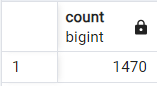
\includegraphics[width=0.4\textwidth]{images/query1.png}
    \caption{Query 1}
    \label{fig:query1}
\end{figure}

\subsection{Query 2}
The count of records for each JobRole in descending order of count
\begin{verbatim}
    SELECT jobrole, COUNT(*) as countrole
    FROM employeeattrition1
    GROUP BY jobrole
    ORDER BY countrole DESC
\end{verbatim}

\begin{figure}[H]
    \centering
    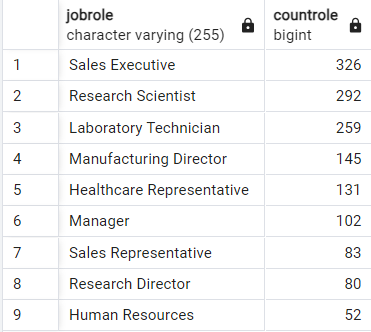
\includegraphics[width=0.6\textwidth]{images/query2.png}
    \caption{Query 2}
    \label{fig:query2}
\end{figure}

\subsection{Query 3}
The average MonthlyIncome and PercentSalaryHike for each JobRole in ascending
order of JobRole
\begin{verbatim}
    SELECT jobrole, AVG(monthlyincome) as avgincome,
    AVG(percentsalaryhike) as avghike
    FROM employeeattrition1
    GROUP BY jobrole
    ORDER BY jobrole
\end{verbatim}

\begin{figure}[H]
    \centering
    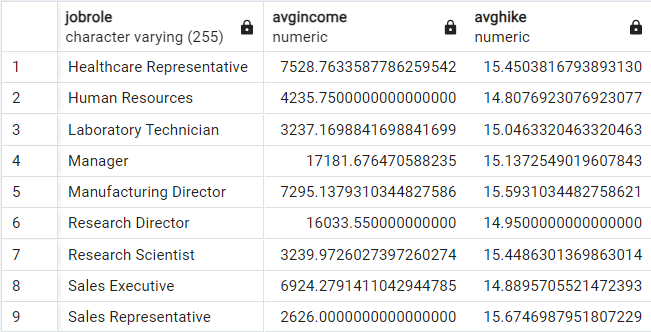
\includegraphics[width=1\textwidth]{images/query3.png}
    \caption{Query 3}
    \label{fig:query3}
\end{figure}

We can see that the average \texttt{PercentSalaryHike} is almost the same for
all the \texttt{JobRole}. However, the average \texttt{MonthlyIncome} is
dependent on the \texttt{JobRole} with \texttt{Manager} having the highest
average \texttt{MonthlyIncome} and \texttt{Sales Representative} having the
lowest average \texttt{MonthlyIncome}.

\subsection{Query 4}
The average JobSatisfaction for each Gender and MaritalStatus
\begin{verbatim}
    SELECT gender, maritalstatus, AVG(jobsatisfaction)
    as avgsat FROM employeeattrition1
    GROUP BY gender, maritalstatus
\end{verbatim}

\begin{figure}[H]
    \centering
    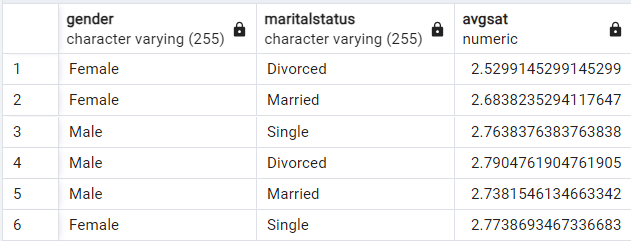
\includegraphics[width=1\textwidth]{images/query4.png}
    \caption{Query 4}
    \label{fig:query4}
\end{figure}

The average \texttt{JobSatisfaction} is almost the same for all the groups
ranging from 2.7 to 2.8. However, the average \texttt{JobSatisfaction} of
\texttt{Divorced Females} is slightly lower at 2.5.

\subsection{Query 5}
The range(Min and Max) of Age and HourlyRate for each JobRole
\begin{verbatim}
    SELECT jobrole,
    min(age) as minage, max(age) as maxage,
    min(hourlyrate) as minrate, max(hourlyrate) as maxrate
    FROM employeeattrition1
    GROUP BY jobrole
\end{verbatim}

\begin{figure}[H]
    \centering
    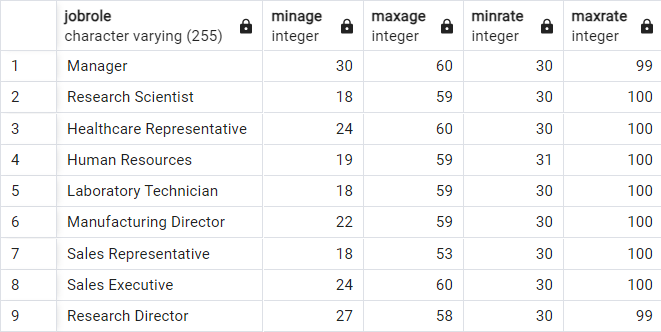
\includegraphics[width=1\textwidth]{images/query5.png}
    \caption{Query 5}
    \label{fig:query5}
\end{figure}

We see that the max \texttt{Age} is about 60 for all the \texttt{JobRole}
except \texttt{Sales Representative} which is 53. The min \texttt{Age} is
around 18 for all the low level \texttt{JobRole} with the exception of
\texttt{Healthcare Representative} which is 24. The min \texttt{Age} for higher
level \texttt{JobRole} start from 22 for \texttt{Manufacturing Director} and
for \texttt{Manager} it is 30.

The min and max \texttt{HourlyRate} is pretty much the same for all the
\texttt{JobRole} with min \texttt{HourlyRate} being around 30 and max
\texttt{HourlyRate} being about 100.

\subsection{Query 6}
Join two tables for \texttt{EmployeeAttrition1.csv} and
\texttt{EmployeeAttrition2.csv} and display 20 records with the following
columns
\begin{enumerate}
    \item EmployeeNumber
    \item Age
    \item Gender
    \item JobRole
    \item OverTime
    \item Attrition
\end{enumerate}
\begin{verbatim}
    SELECT e1.employeenumber, e1.age, e1.gender, e1.jobrole,
    e2.overtime, e2.attrition
    FROM employeeattrition1 e1 JOIN employeeattrition2 e2
    on e1.employeenumber = e2.employeenumber limit 20
\end{verbatim}

\begin{figure}[H]
    \centering
    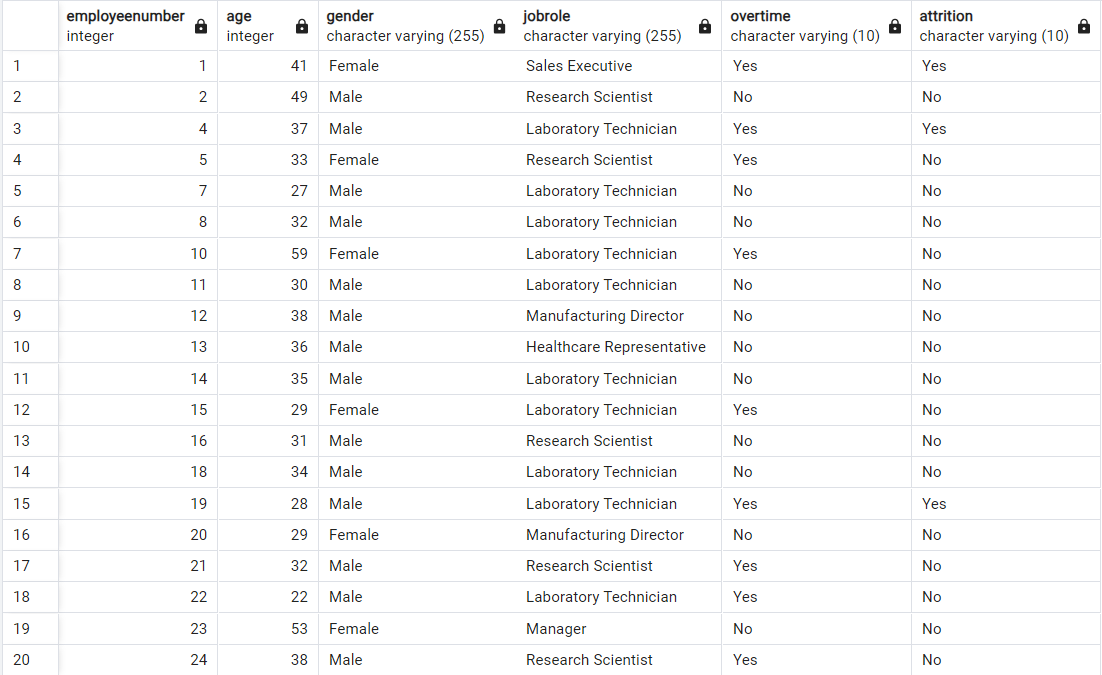
\includegraphics[width=1\textwidth]{images/query6.png}
    \caption{Query 6}
    \label{fig:query6}
\end{figure}
\end{document}